\let\negmedspace\undefined
\let\negthickspace\undefined
\documentclass[journal]{article}
\usepackage[a5paper, margin=10mm, onecolumn]{geometry}
\usepackage{lmodern} % Ensure lmodern is loaded for pdflatex

\setlength{\headheight}{1cm} % Set the height of the header box
\setlength{\headsep}{0mm}     % Set the distance between the header box and the top of the text

\usepackage{gvv-book}
\usepackage{gvv}
\usepackage{cite}
\usepackage{textcomp}
\usepackage{amsmath,amssymb,amsfonts,amsthm}
\usepackage{algorithmic}
\usepackage{graphicx}
\graphicspath{{./figs/}}
\usepackage{textcomp}
\usepackage{xcolor}
\usepackage{txfonts}
\usepackage{listings}
\usepackage{enumitem}
\usepackage{mathtools}
\usepackage{gensymb}
\usepackage{comment}
\usepackage[breaklinks=true]{hyperref}
\usepackage{tkz-euclide} 
\usepackage{listings}
\usepackage{gvv}                                        
\def\inputGnumericTable{}                                 
\usepackage[latin1]{inputenc}                                
\usepackage{color}                                            
\usepackage{array}                                            
\usepackage{longtable}                                       
\usepackage{calc}                                             
\usepackage{multirow}                                         
\usepackage{hhline}                                           
\usepackage{ifthen}                                           
\usepackage{lscape}
\usepackage{circuitikz}
\tikzstyle{block} = [rectangle, draw, fill=blue!20, 
text width=4em, text centered, rounded corners, minimum height=3em]
\tikzstyle{sum} = [draw, fill=blue!10, circle, minimum size=1cm, node distance=1.5cm]
\tikzstyle{input} = [coordinate]
\tikzstyle{output} = [coordinate]


\begin{document}
	
	\bibliographystyle{IEEEtran}
	\vspace{3cm}
	
\title{2.5.1}
\author{EE25BTECH11047 - RAVULA SHASHANK REDDY}
\maketitle
\hrulefill
\bigskip 

\renewcommand{\thetable}{\theenumi}
\setlength{\intextsep}{10pt}
\textbf{Question:} \\

Check whether the points \( (7,10),\; (-2,5),\; (3,4) \) form an isosceles right triangle.\\

\textbf{Solution:}\\

Given:
\begin{align}
\vec{A} = \myvec{7 \\ 10} \\
\vec{B} = \myvec{-2 \\ 5} \\
\vec{C} = \myvec{3 \\ 4}
\end{align}

Side vectors:
\begin{align}
\vec{A}-\vec{B} &= \myvec{7 \\ 10} - \myvec{-2 \\ 5} = \myvec{9 \\ 5} \\
\vec{A}-\vec{C} &= \myvec{7 \\ 10} - \myvec{3 \\ 4} = \myvec{4 \\ 6} \\
\vec{B}-\vec{C} &= \myvec{-2 \\ 5} - \myvec{3 \\ 4} = \myvec{-5 \\ 1}
\end{align}
\newpage
Isosceles check:\\

1. Altitude from $\vec{A}$ 
\begin{align}
\vec{D}=\frac{\vec{B}+\vec{C}}{2}
=\frac{1}{2}\myvec{-2+3\\5+4}
=\myvec{\tfrac{1}{2}\\\tfrac{9}{2}}.\\
\vec{A}-\vec{D}
=\myvec{\tfrac{13}{2}\\\tfrac{11}{2}},\qquad
\vec{B}-\vec{C}
=\myvec{-5\\1}.\\
(\vec{A}-\vec{D})^{T}(\vec{B}-\vec{C})
=\myvec{\tfrac{13}{2} & \tfrac{11}{2}}
\myvec{-5\\1}
=-\tfrac{65}{2}+\tfrac{11}{2}\neq 0.
\end{align}


2. Altitude from $\vec{B}$
\begin{align}
\vec{E}=\frac{\vec{C}+\vec{A}}{2}
=\myvec{5\\7}.\\
\vec{B}-\vec{E}=\myvec{-7\\-2},\qquad
\vec{C}-\vec{A}=\myvec{-4\\-6}.\\
(\vec{B}-\vec{E})^{T}(\vec{C}-\vec{A})
=\myvec{-7 & -2}\myvec{-4\\-6}
=28+12=40\neq 0.
\end{align}
 

3.Altitude from $\vec{C}$
\begin{align}
\vec{F}=\frac{\vec{A}+\vec{B}}{2}
=\myvec{\tfrac{5}{2}\\\tfrac{15}{2}}.\\
\vec{C}-\vec{F}=\myvec{\tfrac{1}{2}\\-\tfrac{7}{2}},\qquad
\vec{A}-\vec{B}=\myvec{9\\5}.\\
(\vec{C}-\vec{F})^{T}(\vec{A}-\vec{B})
=\myvec{\tfrac{1}{2} & -\tfrac{7}{2}}
\myvec{9\\5}
=\tfrac{9}{2}-\tfrac{35}{2}=-13\neq0.
\end{align}
\begin{center}    
Hence it is not isosceles triangle.
\end{center}

Right angle check:\\

For a right angle, the dot product of two sides must be zero.
\begin{align}
(\vec{A}-\vec{B})^T(\vec{A}-\vec{C}) &= (9)(4) + (5)(6) = 66 \neq 0 \\
(\vec{A}-\vec{B})^T(\vec{B}-\vec{C}) &= (9)(-5) + (5)(1) = -40 \neq 0 \\
(\vec{A}-\vec{C})^T(\vec{B}-\vec{C}) &= (4)(-5) + (6)(1) = -14 \neq 0
\end{align}

Hence, the given points forms neither an isosceles nor a right-angled triangle.
\newpage
\begin{figure}
    \centering
    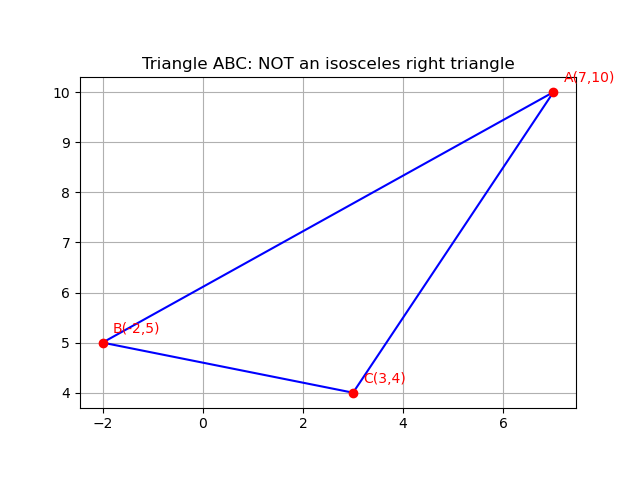
\includegraphics[width=1.0\linewidth]{fig1.png}
    \caption{}
    \label{fig:placeholder}
\end{figure}
\end{document}